\documentclass[a4paper,10pt]{article}
\usepackage[utf8]{inputenc}
\usepackage{color}
\usepackage{listings}
\lstset{language=C}
\usepackage{hyperref}
\usepackage{amsmath}
\usepackage{amssymb}
\usepackage{textcomp}
\usepackage[mathlines]{lineno}
\usepackage{graphicx}
\usepackage[american]{babel}
\usepackage{afterpage}
\usepackage{grffile} 
\usepackage{siunitx} 
\usepackage{multirow}
\usepackage{subcaption} 
\newcommand{\vphi}{\mbox{\boldmath{$\phi$}}}
\newcommand{\vc}{\mbox{\boldmath{$c$}}}
\newcommand{\vmu}{\mbox{\boldmath{$\mu$}}}
\bibliographystyle{mmta}
\usepackage[toc,page]{appendix}
% \usepackage{movie15}
\usepackage{adjustbox}
\usepackage{array}
\usepackage{bm}
\usepackage{xcolor}
\usepackage{tikz}
\usepackage{tikz-3dplot}
\usetikzlibrary{calc}
\usetikzlibrary{plotmarks}
\usepackage{pgfplots}
\usepackage{etoolbox}

\newcommand{\Depth}{2}
\newcommand{\Height}{2}
\newcommand{\Width}{2}

\tdplotsetmaincoords{60}{115}
\pgfplotsset{compat=newest}

%opening
\title{Manual for using the finite difference solver based on the grand-potential formalism}
\author{Abhik Choudhury}
\lstset{
  basicstyle=\ttfamily,
  columns=fullflexible,
  frame=single,
  breaklines=true,
  postbreak=\mbox{\textcolor{red}{$\hookrightarrow$}\space},
}


\begin{document}

\maketitle

\section{Introduction}
This is a multi-phase multicomponent phase-field solver based on a
regular-grid finite-difference discretization, with a
simple Euler forward time marching scheme. It is based on the 
phase-field model presented in \textit{Phys. Rev. E 85, 021602 (2012)}.
The solver is parallelized using a simple domain-decomposition in 
one direction using MPI interface. Before, you run the solver there
are certain basic operations one needs to carry out.

\section{Infile}
The input parameters required for the solver are derived from an 
infile. This contains information about the domain geometry, 
the thermodynamic functions(free energy), material properties 
such as the interfacial energies and their anisotropies 
as well as boundary conditions. It could also contain special
flags related to the running of the solver. The following is a basic 
description of the keys in the infile. \textbf{Each key must end with 
a semicolon}. Additionally, all lines beginning with "\#" will be treated
as comments in the infile.
\lstinputlisting{../Input.in}

\subsection{Simulation geometry, spatial and temporal discretization}

\begin{lstlisting}
##Geometrical dimensions of the simulation domain
DIMENSION = 2;
MESH_X = 100;
MESH_Y = 100;
MESH_Z = 1;
\end{lstlisting}

\begin{itemize}
\item DIMENSION: This can take values 2,3 for 2D and 3D simulations respectively. This is a required key in the solver and not mentioning this key might lead to unexpected results
\item MESH\_X,MESH\_Y,MESH\_Z: These are the number of grid points in the domain(and not the physical lengths) in the respective X, Y, Z directions. 
When DIMENSION is 2, the value of MESH\_Z will redundant and will be taken as 1.
\end{itemize}

\begin{lstlisting}
##Discretization, space and time
DELTA_X = 2.0;
DELTA_Y = 2.0;
DELTA_Z = 2.0;
DELTA_t = 0.08;
\end{lstlisting}

\begin{itemize}
 \item The values DELTA\_X, DELTA\_Y, DELTA\_Z correspond to the grid resolution in the X, Y, Z directions respectively. Similarly, DELTA\_t corresponds to the temporal discretization(time-step).
\end{itemize}

\subsection{Phases and Components information}

\begin{lstlisting}
##Number of phases and composition
NUMPHASES = 2;
NUMCOMPONENTS = 2;
\end{lstlisting}

\begin{itemize}
 \item The keys are self-explanatory. NUMPHASES corresponds to the number of phases in the domain, while NUMCOMPONENTS corresponds to the number of components(2, for binary, 3 for ternary etc.)
 \item These keys are absolutely necessary, please fill carefully for successful running of your codes.
\end{itemize}

\begin{lstlisting}
COMPONENTS = {Al, Cu};
PHASES = {alpha, beta};
\end{lstlisting}

\begin{itemize}
 \item COMPONENTS refers to the tuple that consists of the names of the components. The names are separated by commas and the entire tuple needs to placed within \{\} followed by a semicolon.
 \item Similarly, PHASES refers to the names of the phases in the domain.
\end{itemize}

\subsection{Boundary conditions}

\begin{lstlisting}
##0:FREE, 1: Neumann, 2: Dirichlet, 3: Periodic, 4: Complex
##BOUNDARY = {TYPE, X_LEFT, X_RIGHT, Y_FRONT, Y_BACK, Z_TOP, Z_BOTTOM}
BOUNDARY = {phi, 1, 1, 1, 1, 0, 0};
BOUNDARY = {mu, 1, 1, 1, 1, 0, 0};
BOUNDARY = {c, 1, 1, 1, 1, 0, 0};
BOUNDARY = {T, 1, 1, 1, 1, 0, 0};
\end{lstlisting}

\begin{itemize}
 \item Any of the solvers in repository will consist of the following scalar default types. Type "phi" will represent the phase-field order parameters whose number is specified by the key, "NUMPHASES". 
 Depending on the solver whether it is the grand-potential based solver, where "mu" will be the independent variable or if it is the Cahn-Hilliard or Kim-Kim-Suzuki based solvers, 
 where "c" is the independent variable, Type "mu" or "c" will refer to the components in the key "COMPONENTS". Similarly, type "T" will refer to the temperature field. The BOUNDARY key will refer to the 
 boundary condition for the respective Type of field. The following numbers in a given tuple refer to the boundary at the respective (X\_LEFT, X\_RIGHT, Y\_FRONT, Y\_BACK, Z\_TOP, Z\_BOTTOM) boundaries, 
 that refer to the X, Y, Z boundaries in order. The boundary condition is specified by numbers, 0:FREE, 1: Neumann, 2: Dirichlet, 3: Periodic, 4: Complex, where for the DIRICHLET boundary condition the 
 respective boundary can also take in a specified value which can be specified in the following key: BOUNDARY\_VALUE. If the key is not present, the default remains the one that is initialized at the 
 start of the simulation and is left unchanged. Further, if for any direction, for eg: X, one of the extremeties is specified as a PERIODIC boundary, then the other X-boundary will also be initialized as 
 PERIODIC irrespective of the entry in the tuple. 
\end{itemize}

\begin{lstlisting}
#BOUNDARY_VALUE = {Type, Value X+, Value X-, Value Y+, Value Y-,Value Z+, Value Z-}
BOUNDARY_VALUE = {phi, 0, 0, 0, 0, 0, 0};
BOUNDARY_VALUE = {mu, 0, 0, 0, 0, 0, 0};
BOUNDARY_VALUE = {c, 0, 0, 0, 0, 0, 0};
BOUNDARY_VALUE = {T, 0, 0, 0, 0, 0, 0};
\end{lstlisting}

\begin{itemize}
 \item This key corresponds to a specific value that needs to be specified on a boundary which will be held constant during the duration of the simulation. The definition of this key should 
 follow the BOUNDARY specification and follows the same type of definition, except here the tuple Value X\_LEFT, Value X\_RIGHT, Value Y\_FRONT, Value Y\_BACK, Value Z\_TOP, Value Z\_BOTTOM, refer
 to values on the respective boundaries. The values in this tuple will only be utilized if the respective boundary condition on that boundary is DIRICHLET. By default, the value will be treated as 
 the same as the one that is initialised at the start of the simulation, which will be utilized if this key is not present. 
\end{itemize}

\subsection{Number of iterations, smoothing time-steps and writing interval}

\begin{lstlisting}
#Running and saving information
NTIMESTEPS = 10000;
NSMOOTH = 10;
SAVET = 1000;
STARTTIME = 6000;
RESTART = 1;
\end{lstlisting}

\begin{itemize}
 \item NTIMESTEPS: Total number of iterations that you wish the solver to run. This is not the total time
 \item NSMOOTH: The number of pre-conditioning steps for smoothening sharp phase-field profiles that are initialised at the start of the simulation
 \item SAVET: Writing interval, i.e, frequency of writing files of the respective fields
 \item STARTTIME: The iteration number from which the simulation will start.
 \item RESTART : This key tells the solver to restart by reading in the files corresponding to STARTTIME. If either of the keys STARTTIME/RESTART are non-zero
 the code will restart after reading in the files corresponding to the value STARTTIME. If STARTTIME = 0 and RESTART = 1, it gives the possibility to start from 
 an already initialized file. This is useful when the filling operations for initialization are time-consuming.
\end{itemize}

\subsection{Material parameters}

\begin{lstlisting}
##Gas constant and molar volume
R = 1.0;
V = 1.0;
\end{lstlisting}

\begin{itemize}
 \item The values "R" and "V" will refer to the gas constant and the molar volume respectively 
\end{itemize}

\begin{lstlisting}
#DIFFUSIVITY={Diagonal:0/1, phase, 11,22,33..(K-1) diagonal elements, 12, 13, 23...(rest of the elements; rowwise)}
DIFFUSIVITY = {1, 0, 1};
\end{lstlisting}

\begin{itemize}
 \item The DIFFUSIVITY key refers to the inter-diffusivity matrix which has the tuple in the following form. The first element can taken in values 0/1, "1" refers to as a diagonal matrix and "0" is a full matrix.
 \item The following element refers to the phase number referring to the phases in the list PHASES. This can take values from 0 to NUMPHASES-1.
 \item The following elements are the values in the inter-diffusivity matrix. The first elements are the diagonal terms in the matrix, while the following 
 elements correspond rowwise to the off-diagonal terms in the diffusivity matrix.
 \item If the first element in the tuple is "1", i.e. the matrix is diagonal irrespective of the number of entries in the tuple only the entries 
 corresponding to the diagonal elements in the matrix will be read in.
\end{itemize}

\begin{lstlisting}
##GAMMA = {12, 13, 14, 23, 24...}
GAMMA = {1.0};
\end{lstlisting}

\begin{itemize}
 \item The GAMMA key refers to the interfacial energy $\gamma_{\alpha\beta}$ between the phases $\alpha\beta$. 
 The elements in tuple correspond to all combination of phases forming the interfaces from the list of phases in PHASES numbered from 0 to NUMPHASES-1.
 \item The elements are numbered in the order ${12,13,14,23,24 \ldots N(N-1)}$, $N=NUMPHASES$ where "12" corresponds to the value of the interfacial energy between phase 1 and 2; $\gamma_{12}$.
 \item In the tuple only combinations $\alpha\beta$ are included where $\alpha<\beta$ as the value of the interfacial energy of the $\alpha\beta$ interface is $\gamma_{\alpha\beta}$ which is the same as 
 $\gamma_{\beta\alpha}$.
 \item Therefore, the total number of elements in the tuple is $\frac{N(N-1)}{2}$.
\end{itemize}

\begin{lstlisting}
#EIGEN_STRAIN = {phase, exx, eyy, ezz, eyz, exz, exy};
EIGEN_STRAIN = {0, 0.01, 0.01, 0.0, 0.0, 0.0, 0.0};
EIGEN_STRAIN = {1, 0.01, 0.01, 0.0, 0.0, 0.0, 0.0};
\end{lstlisting}

\begin{itemize}
 \item The EIGEN\_STRAIN key refers to the eigen-strain tensor in a given phase. The information about the elements of the eigen-strain are derived from the elements in the tuple. 
 \item The first element refers to the phase number in the list PHASES and can take in values from 0 to NUMPHASES-1.
 \item The following elements in tuple are mapped to the eigen-strain matrix in the following order $exx, eyy, ezz, eyz, exz, exy$.
 \item This is an important key required for problems where there are coherent interfaces and the phase transformation is coupled with the stress distribution arising due to coherency strains at the interface.
\end{itemize}


\begin{lstlisting}
#VOIGT_ISOTROPIC = {phase, c11, c12, c44};
VOIGT_ISOTROPIC = {0, 270, 187.5, 125.0};
VOIGT_ISOTROPIC = {1, 270, 187.5, 125.0};
\end{lstlisting}

\begin{itemize}
 \item VOIGT\_ISOTROPIC is the key that refers to the elastic stiffness properties in the Voigt notation for an isotropic material. 
 \item The first element in the tuple refers to the phase which will be a number from 0 to NUMPHASES-1.
 \item The following elements are the values $C11,C12,C44$ in order.
\end{itemize}


\begin{lstlisting}
#VOIGT_CUBIC = {phase, c11, c12, c44};
VOIGT_CUBIC = {0, 270, 187.5, 125.0};
VOIGT_CUBIC = {1, 270, 187.5, 125.0};
\end{lstlisting}

\begin{itemize}
 \item VOIGT\_CUBIC is the key that refers to the elastic stiffness properties in the Voigt notation for a cubic material. 
 \item The first element in the tuple refers to the phase which will be a number from 0 to NUMPHASES-1
 \item The following elements are the values $C11,C12,C44$ in order
\end{itemize}

\begin{lstlisting}
#VOIGT_TETRAGONAL = {phase, c11, c12, c13, c33, c44, c66};
\end{lstlisting}

\begin{itemize}
 \item VOIGT\_TETRAGONAL is the key that refers to the elastic stiffness properties in the Voigt notation for a tetragonal material. 
 \item The first element in the tuple refers to the phase which will be a number from 0 to NUMPHASES-1.
 \item The following elements are the values $C11,C12,C13,C33,C44,C66$ in order.
\end{itemize}

\begin{lstlisting}
BINARY = 1;
DILUTE = 0;
\end{lstlisting}

\begin{itemize}
 \item The keys "BINARY", "TERNARY", "DILUTE" are special flags to the solver allowing for simpler routines in the update of the chemical potential or composition fields.
\end{itemize}

\begin{lstlisting}
##FILEWRITING and OUTPUTTING TO SCREEN
## WRITEFORMAT ASCII/BINARY
##TRACK_PROGRESS: interval of writing out the progress of the simulation to stdout. 
WRITEFORMAT = ASCII;
TRACK_PROGRESS = 10;
\end{lstlisting}

\begin{itemize}
 \item The key WRITEFORMAT mentions the type of the output files to be written. The possible values are ASCII or BINARY that are self-explanatory.
 \item For the case when the type chosen is BINARY, the format is BIG-ENDIAN such that it matches the BINARY type required for PARAVIEW.
 \item TRACK\_PROGRESS is a key that will inform the solver about the frequency with which the progress of the simulation will be written to stdout.
 \item The number can be anything other than 0.
\end{itemize}



\subsection{Model specific parameters}

The following parameters are corresponding to the multi-phase, multi-component grand-potential model formalism as described briefly below:
Order parameter fields $\phi_\alpha$ are utilized for the describing the distribution of the N phases in the system. 
They follow the constraint.
$$
\phi_\alpha \in [0, 1]  \quad \text{and} \quad \sum_{\alpha}^{N} \phi_\alpha = 1.
$$

The grand potential functional reads,
\begin{flalign}
\Omega (T, \mu, \vphi) = \int_{\Omega}^{} \left[ \psi (T, \mu, \vphi) + \epsilon a(\vphi, \nabla \vphi) + \dfrac{w(\vphi)}{\epsilon} \right] d\Omega.
\label{eq:grand_eqn}
\end{flalign}

Here, $\epsilon$ is the width of the diffuse interface, which is chosen such that the smallest feature in the 
resulting morphology is accurately resolved. $w(\vphi)$ is the potential which can be a multi-obstacle or a multi-well 
potential. The formulation for a double obstacle potential is,

\begin{flalign}
w(\vphi) = 
\begin{cases}
 \sum_{\substack{\alpha < \beta \\ \delta \neq \alpha \neq \beta}}^{N, N} \dfrac{16}{\pi^2} \gamma_{\alpha \beta} \phi_\alpha \phi_\beta + \gamma_{\alpha \beta \delta} \phi_\alpha \phi_\beta \phi_\delta & \text{if $ \phi \in [0, 1] $,} \\
\infty & \text{otherwise,}
\end{cases}
\label{Obstacle}
\end{flalign}

while the multi-well potential is of the form;

\begin{flalign}
w(\vphi) = 
\begin{cases}
 \sum_{\substack{\alpha < \beta \\ \delta \neq \alpha \neq \beta}}^{N, N} 9\gamma_{\alpha \beta} \phi_\alpha^{2} \phi_\beta^{2} + \gamma_{\alpha \beta \delta} \phi_\alpha \phi_\beta \phi_\delta
\end{cases}
\label{Well}
\end{flalign}


$\gamma_{\alpha\beta}$ is the isotropic surface energy of the 
the $\alpha-\beta$ interface. $\gamma_{\alpha\beta\delta}$ are third-order terms 
added in order to suppress the adsorption of a third phase at a binary interface. 
$a(\vphi, \nabla \vphi)$ is the gradient energy term and $ \psi (T, \mu, \vphi) $ is the grand potential. 
The anisotropy in the interface energy is incorporated in the gradient energy term as,
\begin{flalign}
 a(\phi, \nabla \phi) = \sum_{\alpha < \beta}^{N, N} \gamma_{\alpha \beta} \left[ a_c(\vec{q}_{\, \alpha \beta}) \right]^2 |\vec{q}_{\, \alpha \beta}|^2,
 \label{Eqn_a}
\end{flalign}
where $ a_c $ is the anisotropy function of the $\alpha$ - $\beta$ interface normal vector $ \vec{q}_{\, \alpha \beta} = \phi_\alpha \nabla \phi_\beta - \phi_\beta \nabla \phi_\alpha $.
For imparting a particular rotation through an arbitrary angle; we have the following form for the anisotropy function;
\begin{flalign}
  a(\phi, \nabla \phi) = \sum_{\alpha < \beta}^{N, N} \gamma_{\alpha \beta} \left[ a_c(\vec{q'}_{\, \alpha \beta}) \right]^2 |\vec{q}_{\, \alpha \beta}|^2,
\end{flalign}

where $\vec{q'}_{\,\alpha\beta}={q_x',q_y',q_z'}$ corresponds to the rotation of the $\vec{q}_{\,\alpha\beta}$ by an arbitrary angle 
given by the rotation matrix $R$.

The evolution equation for the phase-field parameters reads:

\begin{flalign}
\tau \epsilon \frac{\partial \phi_{\alpha}}{\partial t}=& \epsilon\left(\nabla \cdot \frac{\partial a(\phi, \nabla \phi)}{\partial \nabla \phi_{\alpha}}
-\frac{\partial a(\phi, \nabla \phi)}{\partial \phi_{\alpha}}\right) 
-\frac{1}{\epsilon} \frac{\partial w(\phi)}{\partial \phi_{\alpha}}-\frac{\partial \Psi(T, \mu, \phi)}{\partial \phi_{\alpha}}-\lambda,
\label{phi_eqn}
\end{flalign}

where $\tau$ is the relaxation constant which controls the kinetics of the phase 
evolution equation and is interpolated at the interface as $\dfrac{\sum_{\alpha,\beta}^{N,N}\tau_{\alpha\beta}\phi_\alpha\phi_\beta}{\sum_{\alpha,\beta}^{N,N}\phi_\alpha\phi_\beta}$,
$\lambda$ is the Lagrange multiplier 
utilized for imposing the constraint $\sum_{\alpha}^{N} \phi_\alpha = 1$, i.e. the sum of volume fraction of all the phases is 1.


With this information, one can now follow the parameters in the file corresponding to the model

\begin{lstlisting}
#Phase-field parameters; epsilon:interface width; it is not the gradient energy coefficient
epsilon = 8.0;
#Tau = {12, 13, 14, 23, 24...}
Tau = {0.28};
#tau: Constant value for points in the bulk
tau = 1.31;
\end{lstlisting}

\begin{itemize}
 \item "epsilon" is the key that is proportional to the interface width as in Eqn.\ref{eq:grand_eqn}.
 \item Tau is the key that is related to the relaxation of the phase-field equation as detailed in \textit{Phys. Rev. E 85, 021602 (2012)}
 as described in Eqn.\ref{phi_eqn}. The value of the relaxation constants for each of the interfaces $\tau_{\alpha\beta}$ is derived from the 
 tuple similar to the GAMMA key for the interfacial energy, where the elements are arranged in the order ${12,13,14,23,24 \ldots N(N-1)}$, $N=NUMPHASES$,
 where "12" corresponds to the relaxation constant of the interface between the phases 1 and 2; $\tau_{12}$.
 \item In the tuple only combinations $\alpha\beta$ are included where $\alpha<\beta$ as the value of the relaxation constant of the $\alpha\beta$, $\tau_{\alpha\beta}$ 
 is the same as $\tau_{\beta\alpha}$.
 \item Therefore, the total number of elements in the tuple is $\frac{N(N-1)}{2}$.
 \item The value of $\tau$ in Eqn.\ref{phi_eqn} is derived through a weighted average of the form 
 $\dfrac{\sum_{\alpha,\beta}^{N,N}\tau_{\alpha\beta}\phi_\alpha\phi_\beta}{\sum_{\alpha,\beta}^{N,N}\phi_\alpha\phi_\beta}$.
 \item The values of $\tau_{\alpha\beta}$ in the tuple can be chosen according to the thin-interface asymptotic analysis 
performed in \textit{Phys. Rev. E 85, 021602 (2012)}, such that diffusion-controlled growth may be achieved for the solid-liquid interfaces, 
while the lowest value among the two solid-liquid interfaces can be chosen for the solid-solid interface, such that the relaxation of the solid-solid interfaces 
is always faster than the solid-liquid interfaces. 
\item Also, at points where $\sum_{\alpha,\beta}^{N,N}\phi_\alpha\phi_\beta = 0$, the value of $\tau$ is set to the key "tau" in the infile.
\end{itemize}

\begin{lstlisting}
Function_anisotropy = 1;
Anisotropy_type = 4; 
\end{lstlisting}

\begin{itemize}
 \item Function\_anisotropy is the key to relate to the particular form of $a(\vphi, \nabla \vphi)$ that is utilized as the gradient energy function.
 \item For a value of zero, the system is isotropic with respect to the change in the interfacial energy with orientation of the interface normal.
 \item A value of 1 corresponds to a particular function as described in Eqn.\ref{Eqn_a} where the anistropy function is present only in the gradient 
 energy term. There are other possibilities where the anisotropy function may also be incorporated in the potential function $w\left(\vphi\right)$ or a combination of 
 $a(\vphi, \nabla \vphi)$ and $w\left(\vphi\right)$ which will be added on later in the solver.
 \item The key Anisotropy\_type refers to the particular symmetry of the anisotropy. For example a value of 4 implies a four fold anisotropy. This essentially sets the 
 function $a_c\left(\vec{q}_{\,\alpha\beta}\right)$ in Eqn.\ref{Eqn_a}, that for the value Anisotropy\_type=4 reads:
 \begin{align*}
  a_c\left(\vec{q}_{\,\alpha\beta}\right) &= 1-\delta_{\alpha\beta}\left(3-4\dfrac{q_x^{4} + q_y^{4} + q_z^{4}}{\left|\vec{q}_{\,\alpha\beta}\right|^{4}}\right), 
 \end{align*}
  where $\delta_{\alpha\beta}$ is the strength of the anisotropy, while $\vec{q}_{\,\alpha\beta}={q_x,q_y,q_z}$, where $q_{x},q_{y},q_{z}$ are the components 
  of the vector $\vec{q}_{\,\alpha\beta}$.
\end{itemize}

\begin{lstlisting}
##dab = {12, 13, 14, 23, 24...}
dab = {0.04};
\end{lstlisting}

\begin{itemize}
 \item The "dab" key in the infile is relevant in the presence of anisotropy in the interfacial energies when the key Anisotropy\_type=4.
 \item The "dab" key refers to the strength of the interfacial energy anisotropy $\delta_{\alpha\beta}$ between the phases $\alpha\beta$. 
 The elements in tuple correspond to all combination of phases forming the interfaces from the list of phases in PHASES numbered 
 from 0 to NUMPHASES-1.
 \item The elements are numbered in the order ${12,13,14,23,24 \ldots N(N-1)}$, $N=NUMPHASES$ where "12" corresponds to the value of the strength of the interfacial energy 
 anisotropy between phases 1 and 2; $\delta_{12}$.
 \item In the tuple only combinations $\alpha\beta$ are included where $\alpha<\beta$ as the value of the anisotropy strength of the $\alpha\beta$ interface is $\delta_{\alpha\beta}$ which is the same as 
 $\delta_{\beta\alpha}$.
 \item Therefore, the total number of elements in the tuple is $\frac{N(N-1)}{2}$.
\end{itemize}

\begin{lstlisting}
#Rotation_matrix = {0, 1, Euler_x(ang), Euler_y(ang), Euler_z(ang)};
Rotation_matrix = {0, 1, 0, 0, 0};
\end{lstlisting}

\begin{itemize}
 \item The "Rotation\_matrix" key refers to the rotation of the anisotropy function by a given Euler angle description given by $\theta_x, \theta_y,\theta_z$, where $\theta_x$ refers
 to the angle of rotation about X-axis, $\theta_y$ refers to the angle of rotation about Y-axis and $\theta_z$ is the angle of rotation about Z-axis.
 \item The values are taken in as a tuple, where the first two elements correspond to numbers from 0 to NUMPHASES-1 corresponding to combinations of 
 phases that can form an interface. 
 \item This rotation operation will be reflected in the interfacial energy anisotropy of the relevant interface. For example if the first two elements are 0 and 1 then the anisotropy function of the 
 interface between the phases 0 and 1 will be influenced.
 \item The following three elements represent the three Euler angles $\theta_x, \theta_y,\theta_z$, where $\theta_x$ as described before.
\end{itemize}

\begin{lstlisting}
##Potential function
Function_W = 1;
Gamma_abc = {123, 124, 234 ...(N)(N-1)(N-2)};
\end{lstlisting}

\begin{itemize}
 \item The "Function\_W" key represents the potential function $w\left(\vphi\right)$ in Eqn.\ref{eq:grand_eqn}. 
 \item For a value of Function\_W=1, the multi-obstacle potential as given in Eqn.\ref{Obstacle} is selected.
 \item While for Function\_W=2, the multi-well potential as given in Eqn.\ref{Well} is selected.
 \item The tuple Gamma\_abc=\{ \} is a list of third-order terms $\gamma_{\alpha\beta\delta}$ as described in the Eqns.\ref{Obstacle},\ref{Well}.
 \item Only combinations $\alpha\beta\delta$ are considered where $\alpha<\beta<\delta$.
 \item The total number of terms are (N(N-1)(N-2)/6).
\end{itemize}

\begin{lstlisting}
Function_F = 1;
A = {0, 1};
A = {1, 1};
ceq = {0, 0, 0.78125};
ceq = {0, 1, 0.5};
ceq = {1, 1, 0.5};
ceq = {1, 0, 0.5};
cfill = {0, 0, 0.78125};
cfill = {0, 1, 0.5};
cfill = {1, 1, 0.5};
cfill = {1, 0, 0.5};
slopes = {0, 0, 0.45};
slopes = {0, 1, 0.45};
slopes = {1, 0, 0.45};
slopes = {1, 1, 0.45};
\end{lstlisting}

$\psi$ is the grand potential density in Eqn.\ref{eq:grand_eqn}, 
which is obtained at any point as a weighted sum of the the grand potential densities of each phase present at that point, 
\begin{flalign}
\psi = \sum_{\alpha}^{N} h_\alpha(\vphi)\psi^\alpha,
\end{flalign}
where, $ h_\alpha(\vphi) $ is a third order interpolation function that reads,
\begin{flalign}
h_\alpha(\vphi) =  3{\phi_\alpha}^2 - 2{\phi_\alpha}^3 + 2\phi_\alpha \sum_{\substack{ \beta, \gamma \neq \alpha \\ \beta < \gamma }}^{N, N} \phi_\beta \phi_\gamma.
\label{eqn:hphi}
\end{flalign}
$ \psi^\alpha = \psi^\alpha(\mu, T) $ is the grand potential density  of phase $ \alpha $ and can be written as \\
\begin{flalign}
\psi^\alpha(T, \mu) = f^\alpha(c^\alpha(T, \mu)) - \mu c^\alpha(T, \mu),
\end{flalign}
where $ f^\alpha $ is the Helmholtz free energy density per unit volume.
Under constant pressure and volume, $f^\alpha$, the Helmholtz free energy density differs from the Gibbs free energy density by a 
constant. 

\begin{itemize}
 \item The key "Function\_F" refers to the selection of the particular free-energy density per unit volume.
 \item For the value of "Function\_F=1" it refers to the case where a parabolic free-energy density is chosen 
 of the type described in (Trans Indian Inst Met (2015) 68(6):1137–1143), (Current Opinion in Solid State and Materials Science 19 (2015) 287–300), 
 (PHYSICAL REVIEW E 91, 022407 (2015)).
 \item The free-energy density is assumed of the form:
 \begin{align}
  f^{\alpha}\left(\vc\right) &= \dfrac{1}{V_m}\Big(\sum_{i<j}^{K,K}A_{ij}^{\alpha}c_ic_j + \sum_j^{K} B_j^{\alpha} c_j + C^{\alpha}\Big),
  \label{free_energy_density}
 \end{align}
 \item where the coefficients $A^{\alpha}, B^{\alpha}$ and $C^{\alpha}$ are the respective coefficients,
$V_m$ is the molar volume that is assumed equal for all the phases in the present discourse and 
$K$ is the number of independent components.
\item The coefficients $A_{ij}$ are linked to the curvatures of the free-energy curves and hence are 
related to an effective susceptibility. This matrix can be directly
obtained from the databases for real material simulations 
by using the information of the free-energies $G^{\alpha}$ for each of the phases as 
$\left(\dfrac{\partial^2 G^{\alpha}}{\partial c_i\partial c_j}\right)_{\vc^{\alpha}_{eq}}$ 
and $\vc^{\alpha}_{eq}$ are the equilibrium compositions of the components in the 
$\alpha-$phase that is in equilibrium with a given 
phase, which is presently chosen to be the liquid. 

\item Returning to keys as you see in Eqn.\ref{free_energy_density}, the key "A" in the infile 
relates to the matrix $A_{ij}^{\alpha}$ in Eqn.\ref{free_energy_density}. 
\item The first element of the tuple $A=\{\}$, is the number of the phase which can be any number between 0 an NUMPHASES-1, referring to a phase in the list PHASES.
\item This is followed by diagonal values of the matrix $A_{ij}$
\item Thereafter, the tuple contains the off-diagonal values of the matrix $A_{ij}$ in the format $i<j$.
\item Symmetry is utilized for populating the other values $j>i$.

\item Assuming $B_j^{l}$ and $C^{l}$ to be zero for
the liquid phase, the conditions of equilibrium (equal diffusion potential and equal grand-potentials
) allows to determine the other coefficients $B_j^{\alpha}$ and $C^{\alpha}$ for
any of the solid-phases, such that the equilibrium between the solid phase $\alpha$
and the liquid phase is reproduced at the respective equilibrium compositions. 
Thus, one can derive for a given temperature $T_{eq}$,
\begin{align}
 B_{j}^{\alpha} &= 2(A_{jj}^{l}c_{eq,j}^{l} - A_{jj}^{\alpha}c_{eq,j}^{\alpha}) 
 + \sum_{j\neq i}\left(A_{ij}^{\alpha} c_{eq,i}^{\alpha} - A_{ij}^{l} c_{eq,i}^{l}\right)
 \label{Coeff_B}\\
 C^{\alpha}    &= \sum_{i\leq j }\left(A_{ij}^{\alpha} c_{eq,i}^{\alpha}c_{eq,j}^{\alpha} - 
 A_{ij}^{l} c_{eq,i}^{l}c_{eq,j}^{l}\right)
 \label{Coeff_C}
\end{align}

\item Therefore, since the coefficients $B_j$ and $C_j$ may be determined once the coefficients 
$A_{ij}$ and the equilibrium compositions $\vc_{eq,j}$ are specified, we take in the information about 
the equilibrium compositions in the infile. 

\item The key "ceq" refers to the equilibrium compositions of the phases. The considered equilibrium is between the last phase 
NUMPHASES-1 and any of the other phases at the temperature provided in the key "Equilibrium\_temperature" which is the same as "T$_{eq}$" 
in Eqn.\ref{Coeff_B},\ref{Coeff_C}.
\item The first two elements of the tuple "ceq=\{\}" are numbers between 0 and N = NUMPHASES-1, which correspond 
to the list of N phases.
\item Thereafter, the tuple consists in order, the compositions of the K = NUMCOMPONENTS-1 components.
\item The required values are corresponding to all combinations "ceq=$\{a, a, 0, 1\ldots K\}$"
and secondly "ceq=$\{a, N-1, 0, 1\ldots K\}$" where $a\in \left[0,N-1\right]$. The former corresponds
to the composition of the "a" phase in equilibrium with the "N-1" phase, and the latter set 
corresponds to the composition of the "N-1" phase in equilibrium with the "a" phase.
\item The remaining possibilities can be skipped.
\item The key "cfill" is of the same type as "ceq" and is utilized while initializing the domain. It is safe to 
start with having the "cfill" the same as "ceq", unless one wants to start with a supersaturation.

\item For describing the driving force as a result of small
undercoolings, we utilize the slopes of the liquidus $m_i^{l}$ and the solidus $m_{i}^{\alpha}$ , 
which can be introduced from known thermodynamics, and can be incorporated in the construction of the 
respective free-energy densities of the phases.  The equilibrium co-existence 
lines and their variation as a function of temperature are reproduced, 
according to the approximation that the tie-lines are preserved for 
smaller undercoolings, i.e. the change in the phase-coexistence
is assumed to occur in a self-similar manner, such that the resultant 
equilibrium compositions at a given undercooling, also exist along the same initial tie-line.
This is described in the following image,

\begin{figure}[!htbp]
\begin{center}
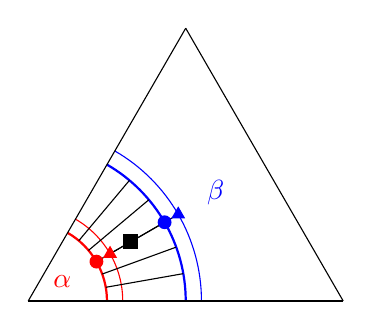
\begin{tikzpicture}[domain=2:4]

\draw [color=red,thick,-] ($(0,0)+(1.0,0)$) 
    arc (0:60:1.0);
\draw [color=blue,thick,-] ($(0,0)+(2.0,0)$) 
    arc (0:60:2.0);
    
\draw [color=red,thin] ($(0,0)+(1.2,0)$) 
    arc (0:60:1.2);
\draw [color=blue,thin] ($(0,0)+(2.2,0)$) 
    arc (0:60:2.2);
    
\pgfmathsetmacro{\XValue}{2.0*cos(20)}%
\pgfmathsetmacro{\YValue}{2.0*sin(20)}%

\pgfmathsetmacro{\xValue}{cos(20)}%
\pgfmathsetmacro{\yValue}{sin(20)}%
% \draw[thin,dashed] (cos(20),sin(20))--(2*cos(20),2*sin(20));
\draw [thin, solid] ($(\xValue,\yValue)$) -- ($(\XValue,\YValue)$);

\pgfmathsetmacro{\XValue}{2.0*cos(10)}%
\pgfmathsetmacro{\YValue}{2.0*sin(10)}%

\pgfmathsetmacro{\xValue}{cos(10)}%
\pgfmathsetmacro{\yValue}{sin(10)}%
% \draw[thin,dashed] (cos(20),sin(20))--(2*cos(20),2*sin(20));
\draw [thin, solid] ($(\xValue,\yValue)$) -- ($(\XValue,\YValue)$);


\pgfmathsetmacro{\XValue}{2.0*cos(30)}%
\pgfmathsetmacro{\YValue}{2.0*sin(30)}%

\pgfmathsetmacro{\xValue}{cos(30)}%
\pgfmathsetmacro{\yValue}{sin(30)}%
% \draw[thin,dashed] (cos(20),sin(20))--(2*cos(20),2*sin(20));
\draw [thin, solid] ($(\xValue,\yValue)$) -- ($(\XValue,\YValue)$);


\pgfmathsetmacro{\XValue}{2.0*cos(40)}%
\pgfmathsetmacro{\YValue}{2.0*sin(40)}%

\pgfmathsetmacro{\xValue}{cos(40)}%
\pgfmathsetmacro{\yValue}{sin(40)}%
% \draw[thin,dashed] (cos(20),sin(20))--(2*cos(20),2*sin(20));
\draw [thin, solid] ($(\xValue,\yValue)$) -- ($(\XValue,\YValue)$);


\pgfmathsetmacro{\XValue}{2.0*cos(50)}%
\pgfmathsetmacro{\YValue}{2.0*sin(50)}%

\pgfmathsetmacro{\xValue}{cos(50)}%
\pgfmathsetmacro{\yValue}{sin(50)}%
% \draw[thin,dashed] (cos(20),sin(20))--(2*cos(20),2*sin(20));
\draw [thin, solid] ($(\xValue,\yValue)$) -- ($(\XValue,\YValue)$);

\pgfmathsetmacro{\xValue}{1.2*cos(30)}%
\pgfmathsetmacro{\yValue}{1.2*sin(30)}%

\pgfmathsetmacro{\XValue}{2.2*cos(30)}%
\pgfmathsetmacro{\YValue}{2.2*sin(30)}%

\draw [thin, solid] ($(\xValue,\yValue)$) -- ($(\XValue,\YValue)$);


\pgfmathsetmacro{\xValue}{cos(30)}%
\pgfmathsetmacro{\yValue}{sin(30)}%

\pgfmathsetmacro{\XValue}{2.0*cos(30)}%
\pgfmathsetmacro{\YValue}{2.0*sin(30)}%

\fill[red] ($(\xValue,\yValue)$) circle(2.5pt);
\fill[blue] ($(\XValue,\YValue)$) circle(2.5pt);

\pgfmathsetmacro{\xValue}{1.2*cos(30)}%
\pgfmathsetmacro{\yValue}{1.2*sin(30)}%

\pgfmathsetmacro{\XValue}{2.2*cos(30)}%
\pgfmathsetmacro{\YValue}{2.2*sin(30)}%

\draw[mark= triangle*,mark size=2.5pt,mark options={color=red}]  plot coordinates {($(\xValue,\yValue)$)};
\draw[mark= triangle*,mark size=2.5pt,mark options={color=blue}] plot coordinates {($(\XValue,\YValue)$)};


\pgfmathsetmacro{\xValue}{1.5*cos(30)}%
\pgfmathsetmacro{\yValue}{1.5*sin(30)}%

\draw[mark=square*,mark size=2.5pt,mark options={color=black}]  plot coordinates {($(\xValue,\yValue)$)};

\pgfmathsetmacro{\xValue}{0.5*cos(30)}%
\pgfmathsetmacro{\yValue}{0.5*sin(30)}%

\pgfmathsetmacro{\XValue}{2.75*cos(30)}%
\pgfmathsetmacro{\YValue}{2.75*sin(30)}%

\node[color=red] at  ($(\xValue, \yValue)$){$\alpha$};
\node[color=blue] at ($(\XValue, \YValue)$){$\beta$};

% \node[mark size=2.5pt,color=blue] at ($(\XValue,\YValue)$) {\pgfuseplotmark{triangle}};

\draw[black] (0,0)--(4,0);
\draw[black] (0,0)--(0.5*4,1.732/2 * 4);
\draw[black] (0.5*4,1.732/2 *4)--(4,0);
%     \draw[color=red] plot[id=x5] function{4*3**0.5 - 3**0.5*x};
% \draw[red] (4.0-0.2,0)--(2-0.2/2, 2*1.732-0.2*1.732/2);
% \fill[red] (3.8*4/5 + 1.9/5, 4*0/5 + 2*1.732/5-0.2*0.2*1.732/2) circle(1.2pt);
% \draw[red,dashed] (4.0-0.3,0)--(2-0.3/2, 2*1.732-0.3*1.732/2);
% \node at (3.7*4/5 + 1.85/5, 4*0/5 + 2*1.732/5-0.3*0.2*1.732/2){$\times$};
% \draw[green] (4.0-1.75,0)--(2-1.75/2, 2*1.732-1.75*1.732/2);
% \fill[green] (2.25*4/5 + 1.125/5, 4*0/5 + 2*1.732/5-1.75*0.2*1.732/2) circle(1.2pt);
% \draw[green,dashed] (4.0-2.0,0)--(2-2.0/2, 2*1.732-2.0*1.732/2);
% \node at (2*4/5 + 1/5, 4*0/5 + 2*1.732/5-2.0*0.2*1.732/2){$\times$};
% %    \draw[blue](3.8*4/5 + 1.9/5, 4*0/5 + 2*1.732/5-0.2*0.2*1.732/2)--(2.25*4/5 + 1.125/5, 4*0/5 + 2*1.732/5-1.75*0.2*1.732/2); 
% \draw[blue](3.8*4/5 + 1.9/5, 4*0/5 + 2*1.732/5-0.2*0.2*1.732/2)--(2*4/5 + 1/5, 4*0/5 + 2*1.732/5-2.0*0.2*1.732/2);
\end{tikzpicture}
\end{center}
\caption{Two-phase equilibrium in a ternary alloy. The phase-co-existence lines at a given temperature 
are drawn as solid curves and the corresponding tie-lines are drawn as solid black lines between the
co-nodes on the co-existence curves. For a particular alloy composition indicated by the solid square, the 
fitting of the free-energies is performed using the equilibrium compositions comprising the tie-line
passing through this point in composition space. For small undercoolings, the change in the phase-co-existence
lines shown as the thin solid lines can be assumed to occur self-similar, such that the resultant 
equilibrium compositions at the undercooled temperature, also exist along the same initial tie-line.}
\label{Tie_line_assumption}
\end{figure}

This allows to write the variation of equilibrium phase concentrations
of both phases $\alpha,l$ as,

\begin{align}
 \dfrac{c_{eq,i}^{\alpha,l}\left(T\right) - c_{eq,i}^{\alpha,l}\left(T_{eq}\right)}{c_{eq,i}^{\alpha}\left(T_{eq}\right) - c_{eq,i}^{l}\left(T_{eq}\right)}&=\dfrac{c_{eq,j}^
 {\alpha,l}\left(T\right)-c_{eq,j}^{\alpha,l}\left(T_{eq}\right)}{c_{eq,j}^
 {\alpha}\left(T_{eq}\right)-c_{eq,j}^{l}\left(T_{eq}\right)} \nonumber\\ 
 &\quad \forall \quad i,j \in 1 \ldots K. 
\end{align}

The extent of extrapolation $\Delta T=(T-T_{eq})$ can be 
expressed as the departure of the 
equilibrium compositions from the chosen 
set at temperature $T_{eq}$,

\begin{align*}
 \sum_{i}m_i^{\alpha,l}\left(c_{eq,i}^{\alpha,l}\left(T\right) - c_{eq,i}^{\alpha,l}\left(T_{eq}\right)\right) = (T-T_{eq}).
\end{align*}

Combining the two preceding relations, we derive 
the equilibrium concentrations of either 
phase as functions of temperature along a given tie-line by, 

\begin{align}
 c_{eq,i}^{\alpha,l}\left(T\right) &= c_{eq,i}^{\alpha,l}\left(T_{eq}\right) + 
 \dfrac{\left(T-T_{eq}\right)\left(c_{eq,i}^{\alpha}\left(T_{eq}\right)-c_{eq,i}^{l}\left(T_{eq}\right)\right)}{\Delta T_f^{\alpha,l}},
\label{phase-compositions}
\end{align}

\noindent
where $\Delta T_f^{\alpha,l}$ is given by,

\begin{align*}
\Delta T_f^{\alpha,l} &= \sum_{i}m_i^{\alpha,l}\left(c_{eq,i}^{\alpha}\left(T_{eq}\right) - c_{eq,i}^{l}\left(T_{eq}\right)\right). 
\end{align*}

Using the above relations for the temperature variations of the equilibrium
compositions of the phases along a chosen tie-line, one can determine the 
coefficients $B_j^{\alpha}\left(T\right)$ and $C^{\alpha}\left(T\right)$ using 
Eqns. \ref{Coeff_B}, \ref{Coeff_C}, such that 
the equilibrium co-existence lines are reproduced for small variations of
both the composition and the temperature around the chosen equilibrium compositions
$\vc_{eq}$ and temperature $T_{eq}$.

\item The required slopes are $m_i^{l}$ and $m_{i}^{\alpha}$ corresponding to the 
equilibrium between the $\alpha$ and the phase $l=N-1$ (the last phase) for the $i^{th}$ component. 
The information is taken from the infile similar to the "ceq" key and the description is as follows;

\item The key "slopes" refers to the slopes of the co-existence curves between phases. The equilibrium is between the last phase 
NUMPHASES-1 and any of the other phases at the temperature provided in the key "Equilibrium\_temperature" which is the same "T$_{eq}$".
\item The first two elements of the tuple "ceq=\{\}" are numbers between 0 and N = NUMPHASES-1, which correspond 
to the list of N phases.
\item Thereafter, the tuple consists in order, the slopes for the K = NUMCOMPONENTS-1 components.
\item The required values are corresponding to all combinations "slopes=$\{a, a, 0, 1\ldots K\}$"
and secondly "slopes=$\{a, N-1, 0, 1\ldots K\}$" where $a\in \left[0,N-1\right]$. The former corresponds
to the slopes of the "a" phase in equilibrium with the "N-1" phase, and the latter set 
corresponds to the slope of the "N-1" phase  in equilibrium with the "a" phase.
For solidification reactions, this would correspond to solidus and liquidus slopes respectively.

\item The remaining possibilities can be skipped.
\end{itemize}

\begin{lstlisting}
##Temperature
ISOTHERMAL = 1;
#Tempgrady={BASETEMP, DELTAT, DISTANCE, OFFSET, VELOCITY}
Tempgrady = {0.96, 0.06, 800.0, 0, 0.016};
Equilibrium_temperature = 1.0;
Filling_temperature = 1.0;
T = 0.96;
\end{lstlisting}

\begin{itemize}
 \item The key "ISOTHERMAL" is flag for the solver setting it for simulations where the temperature "T" will fixed to the value given by the 
 key "T". Setting it to 1 sets the solver up for isothermal simulations.
 \item In the event "ISOTHERMAL=0" the temperature is now not fixed. In the present solver, temperature evolution is not solved yet. 
 However, the option exists to have a non-uniform temperature distribution such as giving a uniform gradient distribution that moves 
 in a particular direction at a perscribed velocity V. This mimics directional solidification conditions. By default the gradient 
 has been defined in the y-direction.
 \item The tuple Tempgrady=\{BASETEMP, DELTAT, DISTANCE, OFFSET, VELOCITY\} is read in for setting the properties of thermal gradient. 
 The first value sets the BASETEMP which is the value at a given location, DELTAT is the temperature increment at a distance given by DISTANCE from the given location(where the 
 temperature was BASETEMP), which sets the magnitude of the thermal gradient. Typically, the BASETEMP is given for the location at y=0. If this is not the 
 case, y=OFFSET is utilized to mention the value of BASETEMP corresponding to y=OFFSET. VELOCITY sets the rate of advance of the linear isotherms in the 
 y-direction corresponding to the imposed value of the directional solidification velocity.
 \item The key "T" sets the value of the temperature for isothermal simulations when the key "ISOTHERMAL = 1".
 \item The key "Equilibrium\_temperature" is the value of "T$_{eq}$" for the equilibrium compositions given in the key "ceq"
and the "slopes" that are defined in the infile. It is this value that is used for determining the phase-compositions as a function of temperature 
as described in Eqn.\ref{phase-compositions}.
\item The key "Filling\_temperature" allows one to use a different temperature for the filling operations concerning the computation of the chemical potential. 
This is useful for non-isothermal simulations when re-starting the simulation from an arbitrary time, by reading from a file. 
\end{itemize}

\begin{lstlisting}
Shift = 0;
ShiftJ = 50;
Writecomposition = 0;
Noise_phasefield = 0;
Amp_Noise_Phase = 0.001;
\end{lstlisting}

\begin{itemize}
 \item The key "Shift" refers to the simulation setting where in the case $\textrm{Shift}=1$ we have all the fields shifted in the negative y-direction
 periodically, as and when the phase boundaries reach the grid-position specified by the key "ShiftJ".
 \item This allows for simulations of infinite growth in the y-direction, relevant for directional solidification, wherein the dynamics in the solid-state
 is zero because of no diffusivity.
 \item "Writecomposition" is a specific key that tells the file-writing function to convert the chemical potential fields into the composition fields and write 
 them along with the chemical potential fields.
 \item "Noise\_phasefield" is a key to impose noise in the phase-field evolution equations at the interface. This is typically utilized for dendritic simulations.
 \item When "Noise\_phasefield=1", the amplitude of the noise is specified by the key "Amp\_Noise\_Phase".
\end{itemize}


\section{Filling}

The instructions about filling the domain with phases present in the file "filling.in", which 
is detailed in \lstinputlisting{../Filling.in}. In the following, the possible filling routines 
are described. The filling instructions may be repeated, that allows for the filling of 
complicated shapes with overlapping. 

\begin{lstlisting}
#FILLCUBE = {phase, x_start, y_start, z_start, x_end, y_end, z_end}
FILLCUBE = {0, 10, 10, 0,  20, 20, 0};
\end{lstlisting}

\begin{itemize}
 \item The "FILLCUBE" key can be utilized for initializing a cube.
 \item The input about the dimensions of the cube are given in the form of a tuple FILLCUBE = \{phase, x\_start, y\_start, z\_start, x\_end, y\_end, z\_end\}, where the 
 first element is a number between 0 and NUMPHASES-1, which indicates a phase in the list PHASES.
 \item The following elements are the co-ordinates(x,y,z) of the end-points of the diagonal in the cube. In the following figure, (x\_start, y\_start, z\_start) corresponds
 to point S and (x\_end, y\_end, z\_end) corresponds to point E in the cube.
 \item This operation leads to the filling of the phase given by the number "phase" in the shape of a cube. All other phases are initialised as zero in this region while the 
 rest of the domain is filled with the last phase NUMPHASES-1.
 \item For 2D object, the z dimensions should be initialised as 0. This would initialize a rectangle.
\end{itemize}


\centering
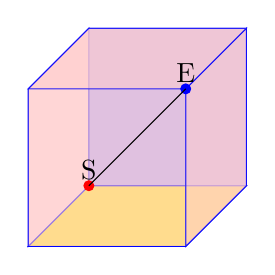
\begin{tikzpicture}
\coordinate (O) at (0,0,0);
\coordinate (A) at (0,\Width,0);
\coordinate (B) at (0,\Width,\Height);
\coordinate (C) at (0,0,\Height);
\coordinate (D) at (\Depth,0,0);
\coordinate (E) at (\Depth,\Width,0);
\coordinate (F) at (\Depth,\Width,\Height);
\coordinate (G) at (\Depth,0,\Height);

\draw[blue,fill=yellow!80] (O) -- (C) -- (G) -- (D) -- cycle;% Bottom Face
\draw[blue,fill=blue!30] (O) -- (A) -- (E) -- (D) -- cycle;% Back Face
\draw[blue,fill=red!10] (O) -- (A) -- (B) -- (C) -- cycle;% Left Face
\draw[blue,fill=red!20,opacity=0.8] (D) -- (E) -- (F) -- (G) -- cycle;% Right Face
\draw[blue,fill=red!20,opacity=0.6] (C) -- (B) -- (F) -- (G) -- cycle;% Front Face
\draw[blue,fill=red!20,opacity=0.8] (A) -- (B) -- (F) -- (E) -- cycle;% Top Face


\fill[red] (0,0,0) circle(2pt);
\node at (0,0.2,0){S};

\fill[blue] (\Depth, \Width, \Height) circle(2pt);
\node at (\Depth, \Width+0.2, \Height){E};

\draw[-,black, thin](0,0,0)--(\Depth, \Width, \Height);

%       \foreach \xy in {O, A, B, C, D, E, F, G}{
%       \node at (\xy) {\xy};
%       }
% \draw[->,>=stealth, thick] (-1,1,1)--(0,1,1);
% \node at (-1,1,1){P};
% \draw[->,>=stealth, thick] (1,-1,1)--(1,0,1);
% \node at (1,-1,1){P};
% \draw[->,>=stealth, thick] (1,1,-1)--(1,1,0);
% \node at (1,1,-1){P};
% 
% \draw[->,>=stealth, thick] (3,1,1)--(2,1,1);
% \node at (3,1,1){P};
% \draw[->,>=stealth, thick] (1,3,1)--(1,2,1);
% \node at (1,3,1){P};
% \draw[->,>=stealth, thick] (1,1,3)--(1,1,2);
% \node at (1,1,3){P};
% 
% \node at (0,1,0) {$L_x$};
% \node at (1,0,0) {$L_y$};
% \node at (0,0,1) {$L_z$};
\end{tikzpicture}

\begin{lstlisting}
##FILLCYLINDER = {phase, x_centre, y_centre, z_start, z_end, radius}
FILLCYLINDER = {0, 50, 50, 0, 0, 20};
\end{lstlisting}

\begin{itemize}
 \item The "FILLCYLINDER" key allows one to initialize a phase in the shape of a cylinder.
 \item The dimensions are provided in the form of a tuple \{phase, x\_centre, y\_centre, z\_start, z\_end, radius\}.
 \item The first element "phase" is a number between 0 and NUMPHASES-1, which indicates a phase in the list PHASES.
 \item The next elements (x\_centre, y\_centre, z\_start) refer to the point S in the following figure.
 \item The next dimension is z\_end which sets the length of the cylinder, i.e the co-ordinate of point E in the following figure is (x\_end, y\_end, z\_end).
 \item Finally, the radius of the cylinder is specified by the final element in the tuple. 
 \item This operation leads to the filling of the phase given by the number "phase" in the shape of a cylinder. All other phases are initialised as zero in this region while the 
 rest of the domain is filled with the last phase NUMPHASES-1.
 \item For 2D object, the z dimensions should be initialised as 0. This would initialize a circle.
 \item Presently, the FILLCYLINDER is designed to fill a cylinder oriented in the Z-direction.
\end{itemize}


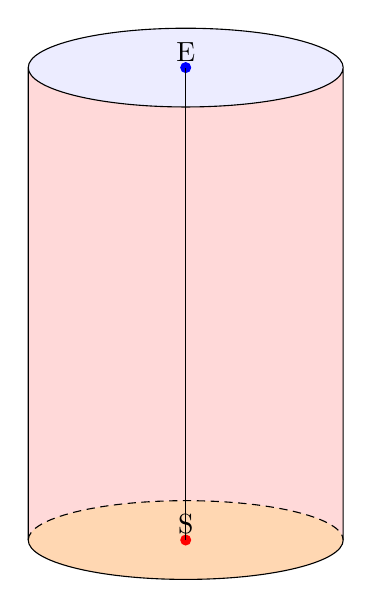
\begin{tikzpicture}
% \fill[top color=blue!50!red,bottom color=red!50,middle color=yellow,opacity=0.25] (0,0) circle (2cm and 0.5cm);
\fill[blue,fill=yellow!80,opacity=0.25] (0,0) circle (2cm and 0.5cm);
% \fill[left color=gray!50!black,right color=gray!50!black,middle color=gray!50,shading=axis,opacity=0.25] (2,0) -- (2,6) arc (360:180:2cm and 0.5cm) -- (-2,0) arc (180:360:2cm and 0.5cm);
\fill[blue,fill=red!60,opacity=0.25] (2,0) -- (2,6) arc (360:180:2cm and 0.5cm) -- (-2,0) arc (180:360:2cm and 0.5cm);
% \fill[top color=gray!90!,bottom color=gray!2,middle color=gray!30,shading=axis,opacity=0.25] (0,6) circle (2cm and 0.5cm);
\fill[blue,fill=blue!30,opacity=0.25] (0,6) circle (2cm and 0.5cm);
\draw (-2,6) -- (-2,0) arc (180:360:2cm and 0.5cm) -- (2,6) ++ (-2,0) circle (2cm and 0.5cm);
\draw[densely dashed] (-2,0) arc (180:0:2cm and 0.5cm);

\fill[red] (0,0,0) circle(2pt);
\node at (0,0.2,0){S};

\fill[blue] (0,6,0) circle(2pt);
\node at (0,6.2,0){E};

\draw[-,black, thin](0,0,0)--(0,6,0);
\end{tikzpicture}


\begin{lstlisting}
#FILLSPHERE = {phase, x_center, y_center, z_center, radius};
FILLSPHERE = {0, 50, 50, 0, 10};
\end{lstlisting}

\begin{itemize}
 \item The "FILLSPHERE" key allows the filling of a phase in the form of a sphere. 
 \item The dimensions are provided in the form of a tuple \{phase, x\_center, y\_center, z\_center, radius\}
 where the first element "phase" is a number from 0 to NUMPHASES-1, which corresponds to a phase in the list PHASES.
 \item The center of the sphere is provided in the next three elements of the tuple (x\_center, y\_center, z\_center).
 \item The last element is the radius of the sphere.
 \item This operation leads to the filling of the phase given by the number "phase" in the shape of a sphere. All other phases are initialised as zero in this region while the 
 rest of the domain is filled with the last phase NUMPHASES-1.
 \item This object can only be used when the DIMENSION = 3 in the infile.
\end{itemize}

\section{Compiling and running}

\begin{itemize}
 \item The solver can be compiled using the command "make" in the command line in a terminal that is opened in the folder which contains the "Makefile".
 \item After compilation the executable "microsim\_gp" will be created. 
 \item The serial solver can be run as ./microsim\_gp name\_of\_infile name\_of\_filling\_file\ name\_of\_output\_file.
 \item The solver takes in three command line arguments, the first is the name of the Input file, the second the name of the filling file containing the information about how the domain 
 should be initialized and thirdly the name of the output file.
 \item The output of the program will be written in a folder "DATA" with the filename "name\_of\_output\_file\_timestep.vtk" for the separate timesteps.
 \item The files at all the timesteps can be opened as a group in the software "paraview" and the fields according to the names given in the COMPONENTS and PHASES keys can be visualized.
 \item As a check the solver also outputs two files "name\_of\_infile.out" and "name\_of\_infile.bd" that prints out the parameters that have been read in by the solver as well as the 
 boundary conditions initialized respectively.
 \item Note, these instructions are presently solver specific. After integration of the software stack, the instructions will get modified slightly.
\end{itemize}


\end{document}
